\documentclass{beamer}

\usetheme{Madrid}
 
\title{\textbf{Introduccióna la Ciencia de Datos}} 
\subtitle{\textbf{Proyecto Final}}
\author{\emph{Procesos migratorios en Cienfuegos}}
\date{\today}

\begin{document}


\begin{frame}
    \titlepage
    \begin{center} 
    \textbf{\large{Autor:}}\\
    \emph{Luis Ernesto Serras Rimada}
    \end{center}
\end{frame}


\begin{frame}{Introducción}
    La búsqueda de mejores oportunidades de empleo y educación es un impulso fundamental que motiva a las personas a migrar, tanto a nivel interno como externo. \\
\begin{itemize}
    \item Este fenómeno refleja no solo la aspiración individual de alcanzar una vida más digna y satisfactoria, sino también un contexto socioeconómico que, en muchos casos, limita el desarrollo personal y profesional en sus lugares de origen.\\
    \item Al mismo tiempo, pone de manifiesto las disparidades entre regiones, donde lugares como La Habana ofrecen un abanico más amplio de oportunidades comparado con provincias como Cienfuegos.\\\\
    \item En última instancia, este deseo de progreso se convierte en una fuerza dinámica que puede transformar realidades, tanto para los individuos como para las comunidades a las que pertenecen.
\end{itemize}
\end{frame}

\section{Recopilación y procesamiento de los Datos}
\begin{frame}
\begin{block}{Datos y su procesamiento}
    \begin{itemize}
        \item La fuente principal de los datos manejados fueron las series estadísticas y anuarios de la \textcolor{blue}{Oficina Nacional de Estadosisticas e Información (ONEI)}.
        \item El análisis en su totalidad fue realizado manejando datos procesados y cargados unicamente desde la manipulación directa de los \textcolor{green}{csv} por medio del módulo de \textcolor{blue}{pandas}.
    \end{itemize}
\end{block}
\end{frame}


\begin{frame}
    \begin{block}{Datos y su procesamiento}
        \begin{itemize}
            Para manejar los datos se hizo uso de la historia de \textcolor{blue}{Perla}, una joven cienfueguera quien (como parte de su desarollo como estudiante de 12mo grado de Preuniversitario, situación familiar y residencial) se enfrenta a los dilemas que se desean exponer, y de esa forma según se avanza en la historia se van presentando los datos visualizandolos de forma natural e interactiva siguiendo su historia.módulo de \textcolor{blue}{pandas}.
        \end{itemize}
    \end{block}

    \begin{center}
        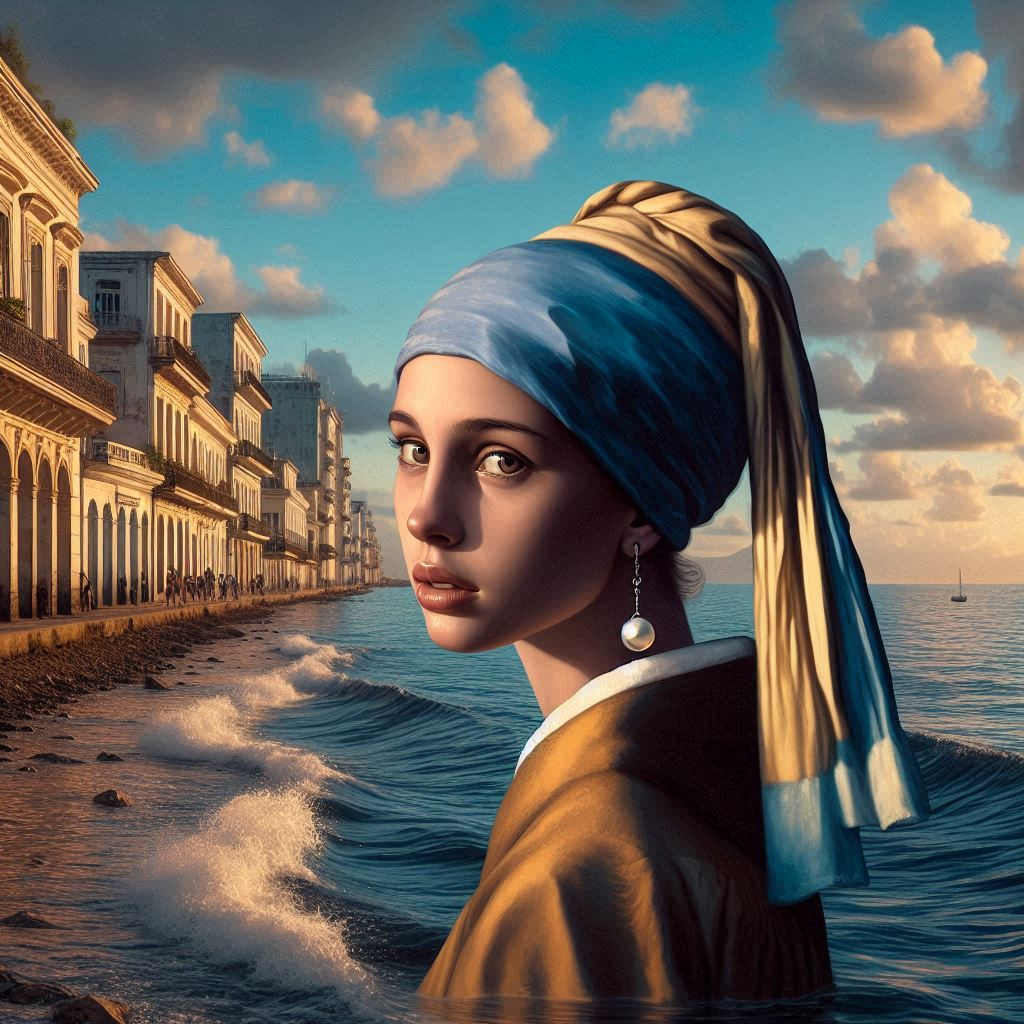
\includegraphics[width=0.5\textwidth]{img/perla4.jpeg}
    \end{center}
\end{frame}
\begin{frame}{Visualizaciones}
    \begin{block}{Población}
    \begin{center}
        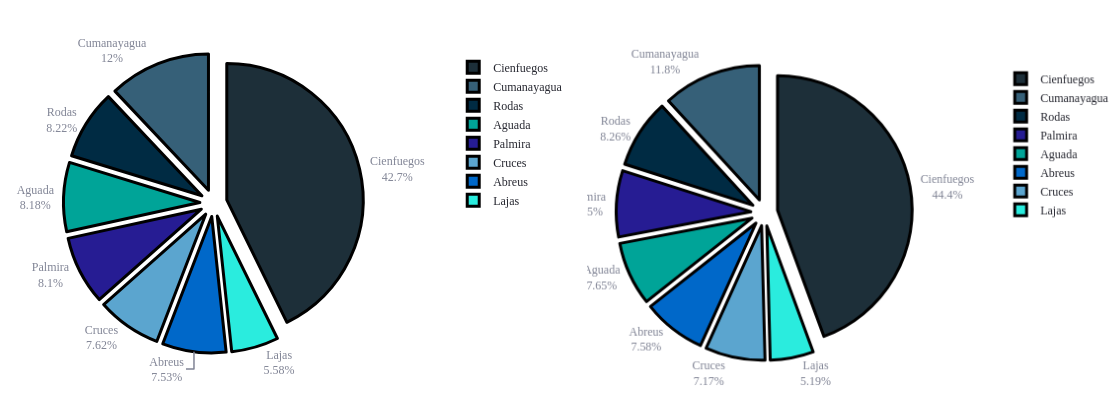
\includegraphics[width=1.0\textwidth]{img/fig1.png}
    \end{center}
    \end{block}
\end{frame}

\begin{frame}
    \begin{block}{Educación Superior}
    \begin{center}
        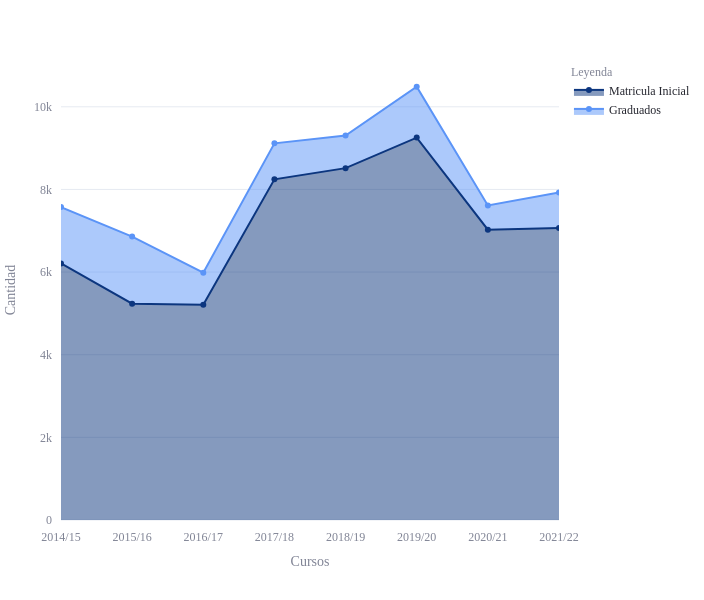
\includegraphics[width=0.8\textwidth]{img/fig2.png}
    \end{center}
    \end{block}
\end{frame}

\begin{frame}
    \begin{block}{Movimientos migratorios}
        \begin{center}
            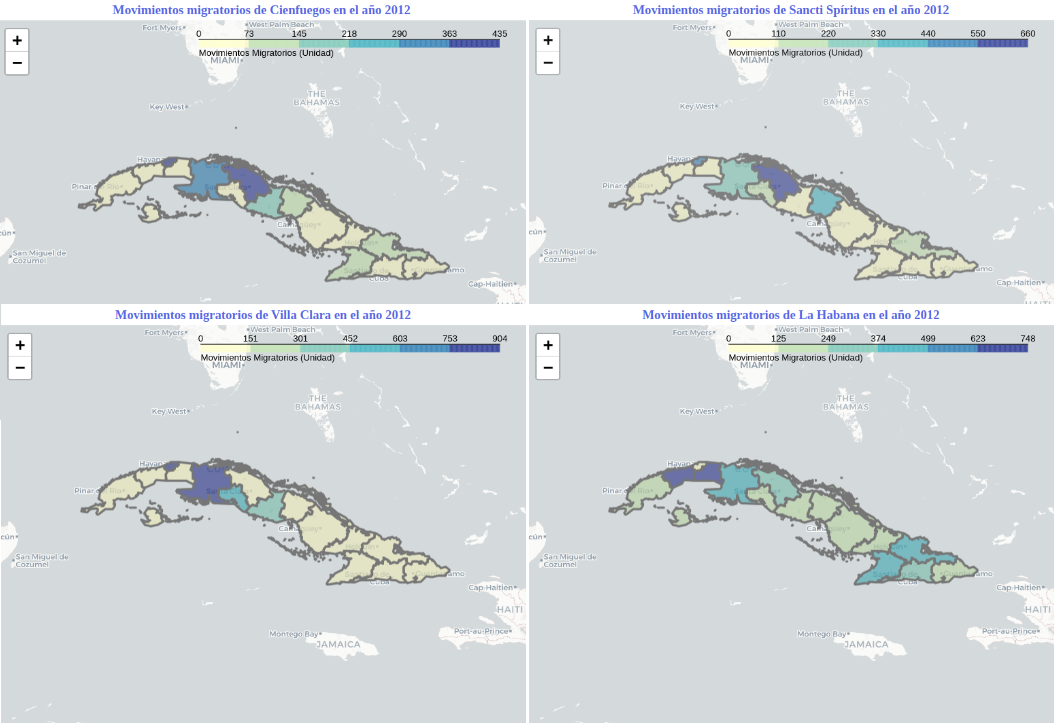
\includegraphics[width=1.0\textwidth]{img/fig3.png}
        \end{center}
    \end{block}
\end{frame}

\begin{frame}
    \begin{block}{Saldo y tasa de migración provincial}
        \begin{center}
            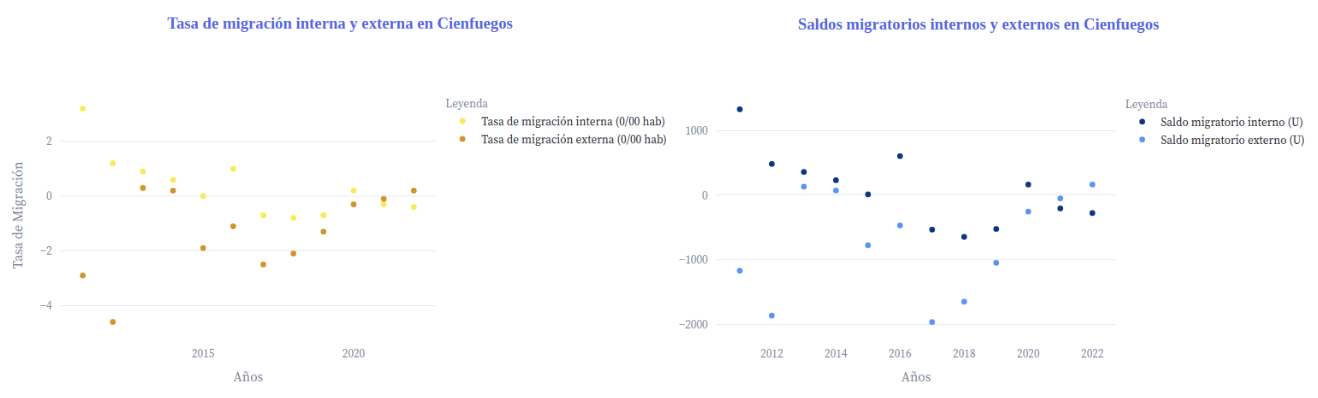
\includegraphics[width=1.0\textwidth]{img/fig4.png}
        \end{center}
    \end{block}
\end{frame}

\begin{frame}
    \begin{block}{Saldo y tasa de migración municipal}
        \begin{center}
            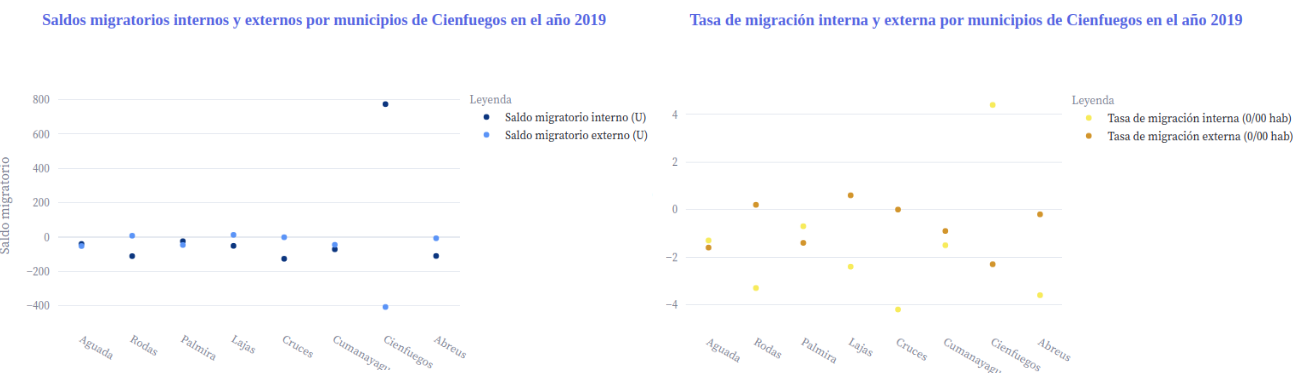
\includegraphics[width=1.0\textwidth]{img/fig5.png}
        \end{center}
        \end{block}
\end{frame}

\begin{frame}
    \begin{block}{Salario medio por provincias}
        \begin{center}
            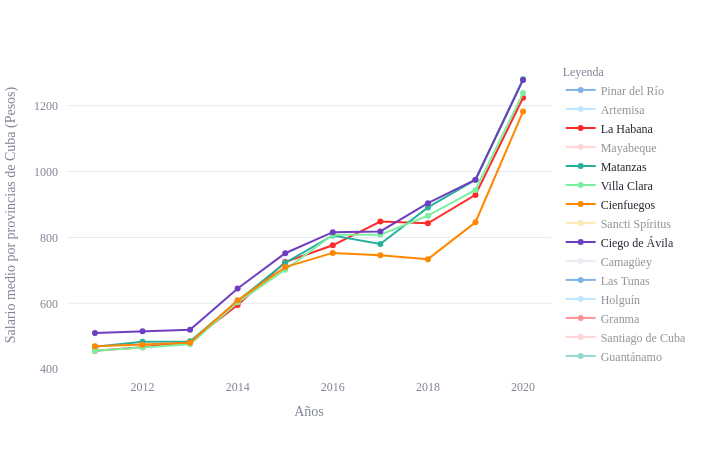
\includegraphics[width=1.0\textwidth]{img/fig6.png}
        \end{center}
    \end{block}
\end{frame}

\begin{frame}
    \begin{block}{Salario medio por municipios}
        \begin{center}
            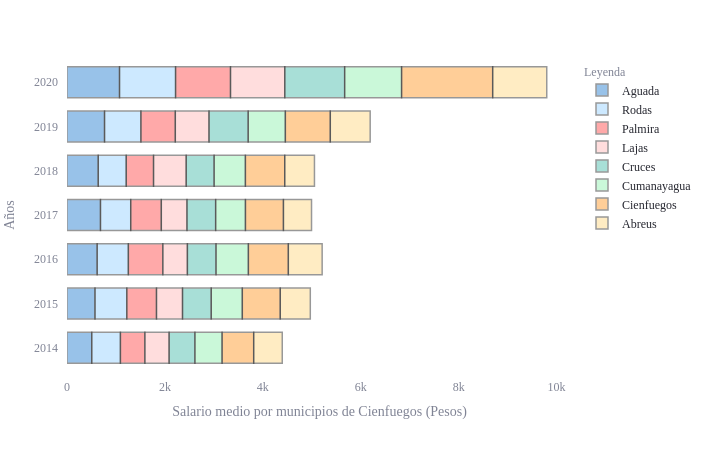
\includegraphics[width=1.0\textwidth]{img/fig7.png}
        \end{center}
    \end{block}
\end{frame}

\begin{frame}
\begin{block}{Fin}
    Muchísimas gracias. :)
\end{block}
\end{frame}
\end{document}